
\documentclass[12pt]{article}
\usepackage{lingmacros}
\usepackage{tree-dvips}
\usepackage{polski}
\usepackage[utf8]{inputenc}
\usepackage{graphicx}
\graphicspath{ {./sprawozdanie-zdjecia/} }
\usepackage[margin=0.5in]{geometry}

\begin{document}

\section*{Sprawozdanie}

\begin{center}
\begin{table}[]
\begin{tabular}{|c|l|}
\hline
\multicolumn{2}{|c|}{Komunikacja człowiek-komputer}                  \\ \hline
\multicolumn{2}{|c|}{Rozpoznawanie pieniędzy}                        \\ \hline
\multicolumn{1}{|l|}{Dominik Doberski 132207} & Artur Olejnik 122402 \\ \hline
\end{tabular}
\end{table}
\end{center}

\subsection*{OVERVIEW}

Celem projektu było stworzenie programu wykrywającego pieniądze na zdjęciach.\\
Należało wykryć:

Monety o nominałach 5gr, 20gr, 2zł, 5zł.

Banknoty o nominałach 20zł, 50zł.
\newpage
\subsection*{KROKI DZIAŁANIA}
Pierwszym krokiem było wykrycie okręgów oraz prostokątów na zdjęciu.
\\Nasze podejście zakładało stworzenie kilku wyspecjalizowanych funkcji wykrywających monety i banknoty zależnie od rodzaju zdjęcia, a następnie zsumowanie ich wyników.\\
Odrzucaliśmy okręgi które są za duże lub większość ich obszaru zajmuje kolor tła.\\
Niektóre z funkcji wykrywały te same monety dlatego odrzucamy kontury które przynajmniej w połowie zawierają się w innych.
\subsubsection*{Hough}
Funkcja wykorzystująca momenty Hougha okazała się nieprzydatna.
W większości przypadków znajdowała okręgi w złych miejscach (najczęściej na banknotach).

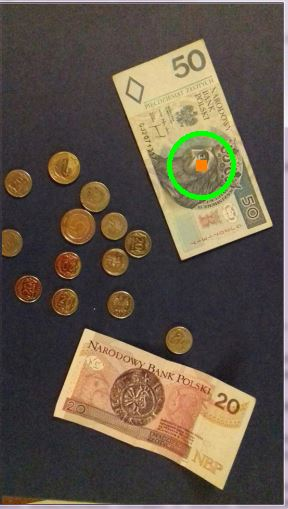
\includegraphics[scale=0.4]{momentyHougha}

W nielicznych przypadkach algorytm był wstanie wykryć monetę poprawnie (moneta oznaczona pomarańczową kropką).

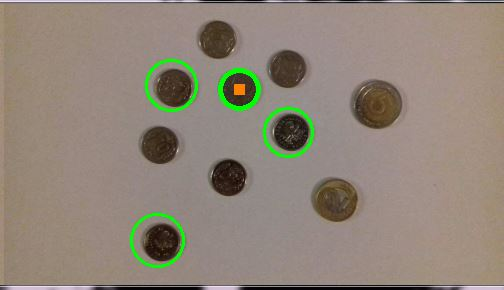
\includegraphics[scale=0.5]{momentyHoughaOK}

Algorytm okazał się tak nieskuteczny, że nie użyliśmy go w ostatecznym rozwiązaniu.
\newpage
\subsubsection*{Adaptive thresholding}
Algorytm adaptive thresholding okazał się przydatny w niektórych przypadkach, szczególnie dobrze nadając się do wykrywania monet na zdjęciach pod kątem.
Najpierw konwertujemy zdjęcie na odcienie szarości.

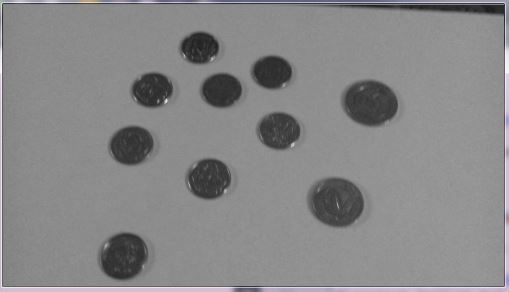
\includegraphics[scale=0.4]{AdaptiveTGray}

Następnie używamy funkcji GaussianBlur aby pozbyć się szczegółów na zdjęciu, monety stają się rozmyte dzięki czemu adaptive treshold nie wyrkywa wzorów na nich.

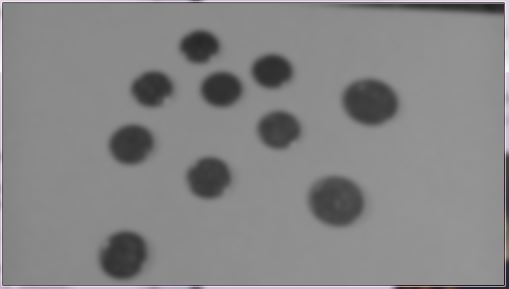
\includegraphics[scale=0.4]{AdaptiveTBlur}

Na tak przygotowanym zdjęciu uruchamiamy algorytm adaptive Tresholding.

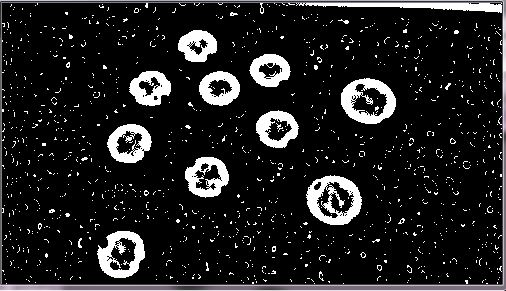
\includegraphics[scale=0.4]{AdaptiveT}

Wykryte kontury zaznaczone okręgami

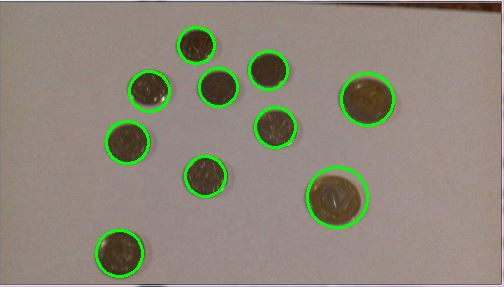
\includegraphics[scale=0.4]{AdaptiveTResult}

Algorytm nie nadaje się gdy tło jest niejednolite (efekt działania przedstawiony na zdjęciu).

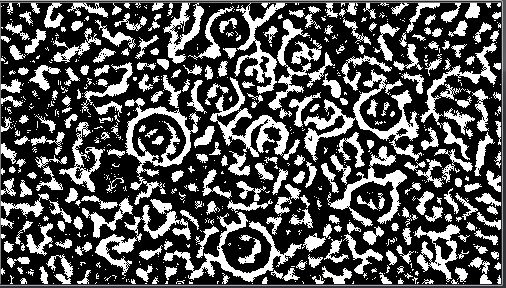
\includegraphics[scale=0.4]{AdaptiveTBad}
\newpage
\subsubsection*{Bright coins}
Aby znaleźć monety szczególnie mocno naświetlone w pierwszej kolejności zmniejszamy jasność i zwiększamy kontrast zdjęcia.

\includegraphics[scale=0.4]{BrightC}

Zamieniamy model kolorów z RGB na HSV aby otrzymać dostęp do zmiennej value która pozwala łatwo odseparować jasne elementy od ciemnych.

\includegraphics[scale=0.4]{BrightV}

Na tak przygotowanym zdjęciu uruchamiamy thresholding i rysujemy okręgi w miejscu wykrytych konturów.

\includegraphics[scale=0.4]{BrightR}

Algorytm mimo, że przygotowany był z myślą o najjaśniejszych monetach skutecznie wykrywa większość monet jakie mamy na zdjęciach.

Dla zbyt ciemnych zdjęć zmniejszona jasność uniemożliwia znalezienie monet.

\includegraphics[scale=0.4]{BrightBad}

\newpage
\subsubsection*{Silver coins}
Kolejny algorytm filtruje srebrne monety na zdjęciu.
W modelu RGB odrzucamy kolory które mają wartości RGB oddalone od siebie o więcej niż 40, zostawiając w ten sposób tylko odcienie szarości. Usuwamy także wartości poniżej 5 (czarny) oraz powyżej 250(biały).

Okazało się jednak, że srebrne monety często na zdjęciach mają kolor bardziej kremowy który nie spełnia naszych założeń, natomiast szaroniebieski kolor na banknocie 50zł nie był usuwany. Niektóre tła z których korzystaliśmy były ciemne przez co nasz algorytm często ich również nie usuwał.

W efekcie z większości zdjęć algorytm usuwał jedynie monety co pozwoliło łatwo je wykrywać.

\includegraphics[scale=0.4]{RemoveSilver}

Treshold uruchomiony na zdjęciu z usuniętymi monetami.

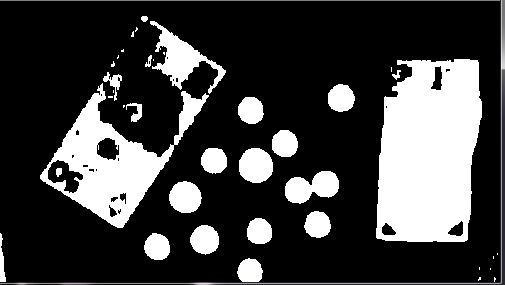
\includegraphics[scale=0.4]{removeSilverTresh}

Wykryte monety.

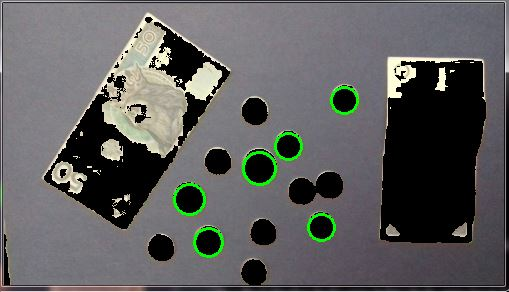
\includegraphics[scale=0.4]{removeSilverResult}

Udało nam się znaleźć jednak zdjęcie z którego usuwane jest tło, a monety po części zostają.

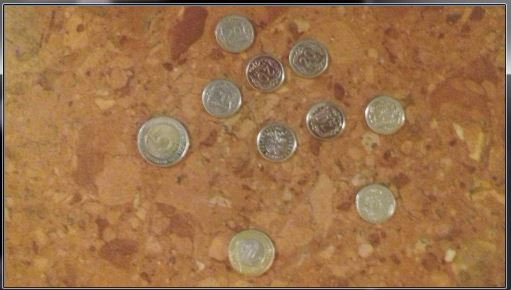
\includegraphics[scale=0.4]{picture_024}
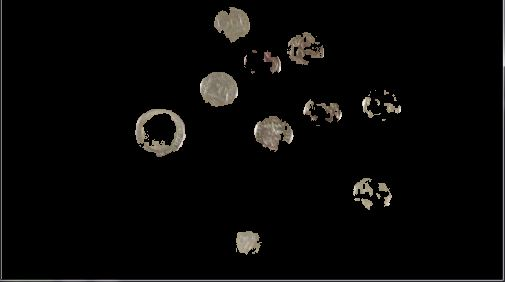
\includegraphics[scale=0.4]{removeNotSilver}

Treshold oraz wykryte kontury.

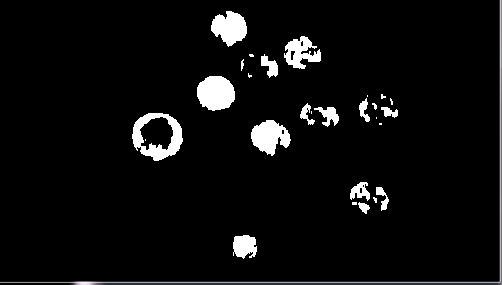
\includegraphics[scale=0.4]{removeNotSilverTresh}
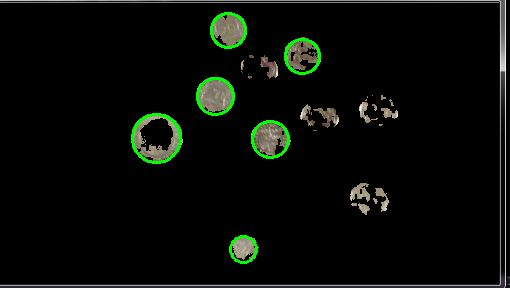
\includegraphics[scale=0.4]{removeNotSilverResult}

\newpage
\subsubsection*{Usuwanie duplikatów}
Dla każdego konturu sprawdzamy czy w liście konturów które rysujemy istnieje taki którego przynajmniej połowa punktów jest wewnątrz danego konturu. Jeżeli tak, zakładamy, że jest to powtórzony kontur i odrzucamy go. W przeciwnym wypadku dodajemy kontur do listy konturów do narysowania.
Do sprawdzenia, czy punkt jest wewnątrz konturu używamy wbudowanej w opencv funkcji pointPolygonTest.

Zdjęcie z narysowanymi wszystkimi konturami wykrytymi przez nasze algorytmy.

\includegraphics[scale=0.8]{wszystkie}

Zdjęcie z odfiltrowanymi konturami (linie na monetach i banknotach są cieńsze - narysowane tylko raz)

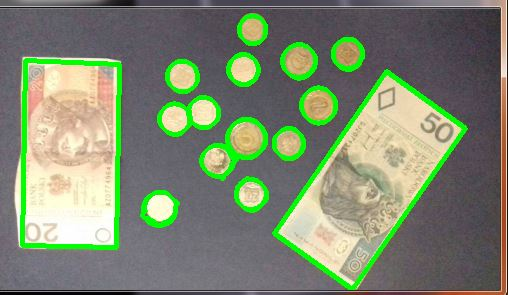
\includegraphics[scale=0.8]{filtrowane}

\newpage
\subsubsection*{Usuwanie elementów wewnątrz banknotów}
Niektóre elementy wewnątrz banknotów mogą być wykrywane jako monety ze względu na kształt przypominający okrąg lub bardzo skupiony kontur. Aby tego uniknąć wykorzystaliśmy funkcję biblioteki opencv, która sprawdza powierzchnię przecięcia dwóch konturów. Okazała się ona być bardzo skuteczna, została ona wykorzystana również przy usuwaniu duplikatów banknotów. Jeśli wyznaczona powierzchnia była większa od zera, wykryta "moneta" została usunięta z pamięci.

Przy użyciu tej metody należy założyć, że monety nie mogą znajdować się na banknotach, ani nawet na ich krawędziach (na przykład w celu podtrzymania banknotu). Problemem może być znajdywanie się monet bardzo blisko banknotu, co przy niedokładnych metodach, które biorą pod uwagę również powierzchnię w pobliżu monety i banknotu, może doprowadzić do eliminowania tych monet. Takie przypadki akurat w naszym przypadku nie zostały jednak zauważone.

Zdjęcie przed użyciem powyższej metody.

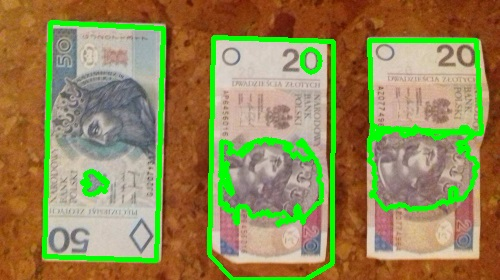
\includegraphics[scale=0.8]{banknoty1}

Zdjęcie po użyciu powyższej metody.

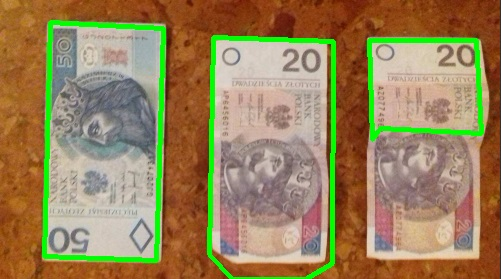
\includegraphics[scale=0.8]{banknoty2}

\newpage
\subsection*{WNIOSKI}
Początkowo próbowaliśmy stworzyć jedną funkcję która wykrywa wszystkie monety na zdjęciu. Takie podejście okazało się błędne, odpowiednio dobrane parametry sprawiały, że funkcja działała tylko dla konkretnego zdjęcia, a dla innych zwraca błędny wynik. 

Przykład błędnie znalezionych okręgów i prostokąta.

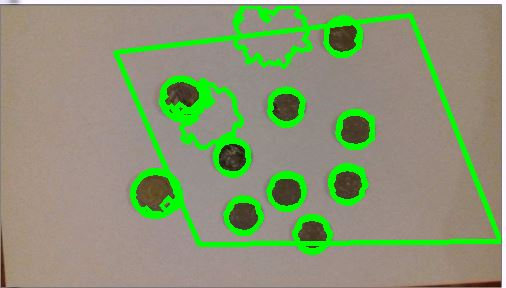
\includegraphics[scale=0.8]{dziwnyRownoleglobok}

Dobrym rozwiązaniem okazało się stworzenie wielu funkcji i wybranie sumy znalezionych konturów co jest zaprezentowane w poprzednim punkcie sprawozdania. 

Aby odfiltrować błędnie znalezione kontury odrzucamy te, które są zbyt duże w stosunku do całego zdjęcia. Odrzucamy również te kontury monet, które pokrywają się z konturami wykrytych banknotów. Ma to na celu wyeliminowanie wykrytych okręgów, które są częścią wzoru banknotu.

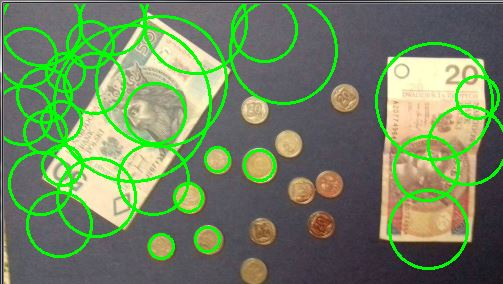
\includegraphics[scale=0.8]{zaduzo}

Odfiltrowane za duże okręgi.

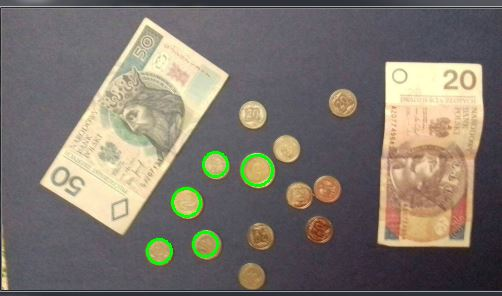
\includegraphics[scale=0.8]{bezzaduzo}

Planujemy odfiltrowywać znalezione kontury, jeżeli większość ich pola ma kolor tła. Ta funkcjonalność nie jest jednak jeszcze zaimplementowana dlatego nie możemy poprzeć jej obrazem.

Wśród posiadanych zdjęć trafiliśmy też na takie, które nie są dobrze rozpoznawane przez żadną z naszych metod, przez co dużo monet pozostaje nierozpoznanych.

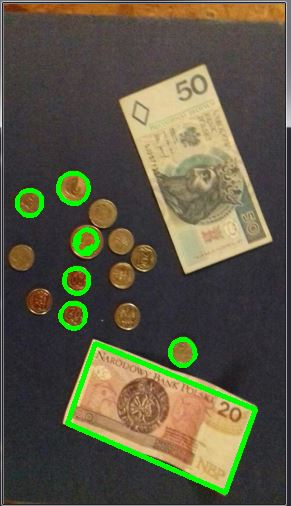
\includegraphics[scale=0.8]{slabe}

Zauważyliśmy, że na różnych zdjęciach takie same monety różnią się od siebie kolorem. Co ciekawe, to samo tyczyło się banknotów. Dodatkowo, niemal na każdym zdjęciu monety są innego koloru niż w rzeczywistości. Widać to na przykładzie opisanej wcześniej funkcji, która miała filtrować kolory inne niż srebrny. Może spowodować to duże problemy z rozpoznaniem monet.

Monety 20 groszowe na różnych zdjęciach.
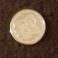
\includegraphics[scale=1]{20gr1}
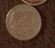
\includegraphics[scale=1]{20gr2}
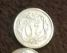
\includegraphics[scale=1]{20gr3}
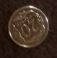
\includegraphics[scale=1]{20gr4}
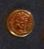
\includegraphics[scale=1]{20gr5}
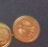
\includegraphics[scale=1]{20gr6}

\newpage
Co gorsze monety mogą różnić się kolorem nawet w obrębie pojedynczego zdjęcia z powodu padającego na nie światła.

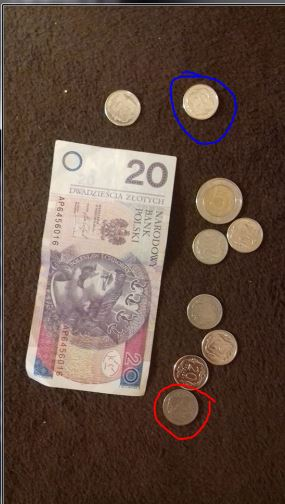
\includegraphics[scale=0.8]{20gr_rozne}

Próbowaliśmy edytować zdjęcie poprzez zmianę kanału "hue" oraz "saturation" w modelu HSV, jednak różnice nadal są wyraźne.

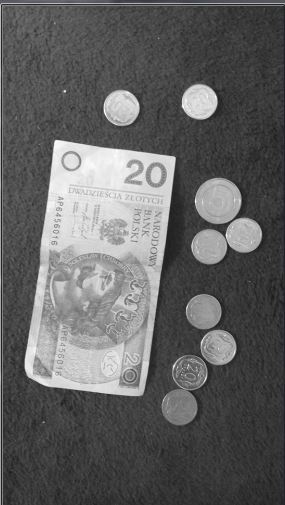
\includegraphics[scale=0.8]{HS}
\end{document}